% Options for packages loaded elsewhere
\PassOptionsToPackage{unicode}{hyperref}
\PassOptionsToPackage{hyphens}{url}
\PassOptionsToPackage{dvipsnames,svgnames,x11names}{xcolor}
%
\documentclass[
  letterpaper,
  DIV=11,
  numbers=noendperiod]{scrartcl}

\usepackage{amsmath,amssymb}
\usepackage{iftex}
\ifPDFTeX
  \usepackage[T1]{fontenc}
  \usepackage[utf8]{inputenc}
  \usepackage{textcomp} % provide euro and other symbols
\else % if luatex or xetex
  \usepackage{unicode-math}
  \defaultfontfeatures{Scale=MatchLowercase}
  \defaultfontfeatures[\rmfamily]{Ligatures=TeX,Scale=1}
\fi
\usepackage{lmodern}
\ifPDFTeX\else  
    % xetex/luatex font selection
\fi
% Use upquote if available, for straight quotes in verbatim environments
\IfFileExists{upquote.sty}{\usepackage{upquote}}{}
\IfFileExists{microtype.sty}{% use microtype if available
  \usepackage[]{microtype}
  \UseMicrotypeSet[protrusion]{basicmath} % disable protrusion for tt fonts
}{}
\makeatletter
\@ifundefined{KOMAClassName}{% if non-KOMA class
  \IfFileExists{parskip.sty}{%
    \usepackage{parskip}
  }{% else
    \setlength{\parindent}{0pt}
    \setlength{\parskip}{6pt plus 2pt minus 1pt}}
}{% if KOMA class
  \KOMAoptions{parskip=half}}
\makeatother
\usepackage{xcolor}
\setlength{\emergencystretch}{3em} % prevent overfull lines
\setcounter{secnumdepth}{5}
% Make \paragraph and \subparagraph free-standing
\makeatletter
\ifx\paragraph\undefined\else
  \let\oldparagraph\paragraph
  \renewcommand{\paragraph}{
    \@ifstar
      \xxxParagraphStar
      \xxxParagraphNoStar
  }
  \newcommand{\xxxParagraphStar}[1]{\oldparagraph*{#1}\mbox{}}
  \newcommand{\xxxParagraphNoStar}[1]{\oldparagraph{#1}\mbox{}}
\fi
\ifx\subparagraph\undefined\else
  \let\oldsubparagraph\subparagraph
  \renewcommand{\subparagraph}{
    \@ifstar
      \xxxSubParagraphStar
      \xxxSubParagraphNoStar
  }
  \newcommand{\xxxSubParagraphStar}[1]{\oldsubparagraph*{#1}\mbox{}}
  \newcommand{\xxxSubParagraphNoStar}[1]{\oldsubparagraph{#1}\mbox{}}
\fi
\makeatother

\usepackage{color}
\usepackage{fancyvrb}
\newcommand{\VerbBar}{|}
\newcommand{\VERB}{\Verb[commandchars=\\\{\}]}
\DefineVerbatimEnvironment{Highlighting}{Verbatim}{commandchars=\\\{\}}
% Add ',fontsize=\small' for more characters per line
\usepackage{framed}
\definecolor{shadecolor}{RGB}{241,243,245}
\newenvironment{Shaded}{\begin{snugshade}}{\end{snugshade}}
\newcommand{\AlertTok}[1]{\textcolor[rgb]{0.68,0.00,0.00}{#1}}
\newcommand{\AnnotationTok}[1]{\textcolor[rgb]{0.37,0.37,0.37}{#1}}
\newcommand{\AttributeTok}[1]{\textcolor[rgb]{0.40,0.45,0.13}{#1}}
\newcommand{\BaseNTok}[1]{\textcolor[rgb]{0.68,0.00,0.00}{#1}}
\newcommand{\BuiltInTok}[1]{\textcolor[rgb]{0.00,0.23,0.31}{#1}}
\newcommand{\CharTok}[1]{\textcolor[rgb]{0.13,0.47,0.30}{#1}}
\newcommand{\CommentTok}[1]{\textcolor[rgb]{0.37,0.37,0.37}{#1}}
\newcommand{\CommentVarTok}[1]{\textcolor[rgb]{0.37,0.37,0.37}{\textit{#1}}}
\newcommand{\ConstantTok}[1]{\textcolor[rgb]{0.56,0.35,0.01}{#1}}
\newcommand{\ControlFlowTok}[1]{\textcolor[rgb]{0.00,0.23,0.31}{\textbf{#1}}}
\newcommand{\DataTypeTok}[1]{\textcolor[rgb]{0.68,0.00,0.00}{#1}}
\newcommand{\DecValTok}[1]{\textcolor[rgb]{0.68,0.00,0.00}{#1}}
\newcommand{\DocumentationTok}[1]{\textcolor[rgb]{0.37,0.37,0.37}{\textit{#1}}}
\newcommand{\ErrorTok}[1]{\textcolor[rgb]{0.68,0.00,0.00}{#1}}
\newcommand{\ExtensionTok}[1]{\textcolor[rgb]{0.00,0.23,0.31}{#1}}
\newcommand{\FloatTok}[1]{\textcolor[rgb]{0.68,0.00,0.00}{#1}}
\newcommand{\FunctionTok}[1]{\textcolor[rgb]{0.28,0.35,0.67}{#1}}
\newcommand{\ImportTok}[1]{\textcolor[rgb]{0.00,0.46,0.62}{#1}}
\newcommand{\InformationTok}[1]{\textcolor[rgb]{0.37,0.37,0.37}{#1}}
\newcommand{\KeywordTok}[1]{\textcolor[rgb]{0.00,0.23,0.31}{\textbf{#1}}}
\newcommand{\NormalTok}[1]{\textcolor[rgb]{0.00,0.23,0.31}{#1}}
\newcommand{\OperatorTok}[1]{\textcolor[rgb]{0.37,0.37,0.37}{#1}}
\newcommand{\OtherTok}[1]{\textcolor[rgb]{0.00,0.23,0.31}{#1}}
\newcommand{\PreprocessorTok}[1]{\textcolor[rgb]{0.68,0.00,0.00}{#1}}
\newcommand{\RegionMarkerTok}[1]{\textcolor[rgb]{0.00,0.23,0.31}{#1}}
\newcommand{\SpecialCharTok}[1]{\textcolor[rgb]{0.37,0.37,0.37}{#1}}
\newcommand{\SpecialStringTok}[1]{\textcolor[rgb]{0.13,0.47,0.30}{#1}}
\newcommand{\StringTok}[1]{\textcolor[rgb]{0.13,0.47,0.30}{#1}}
\newcommand{\VariableTok}[1]{\textcolor[rgb]{0.07,0.07,0.07}{#1}}
\newcommand{\VerbatimStringTok}[1]{\textcolor[rgb]{0.13,0.47,0.30}{#1}}
\newcommand{\WarningTok}[1]{\textcolor[rgb]{0.37,0.37,0.37}{\textit{#1}}}

\providecommand{\tightlist}{%
  \setlength{\itemsep}{0pt}\setlength{\parskip}{0pt}}\usepackage{longtable,booktabs,array}
\usepackage{calc} % for calculating minipage widths
% Correct order of tables after \paragraph or \subparagraph
\usepackage{etoolbox}
\makeatletter
\patchcmd\longtable{\par}{\if@noskipsec\mbox{}\fi\par}{}{}
\makeatother
% Allow footnotes in longtable head/foot
\IfFileExists{footnotehyper.sty}{\usepackage{footnotehyper}}{\usepackage{footnote}}
\makesavenoteenv{longtable}
\usepackage{graphicx}
\makeatletter
\newsavebox\pandoc@box
\newcommand*\pandocbounded[1]{% scales image to fit in text height/width
  \sbox\pandoc@box{#1}%
  \Gscale@div\@tempa{\textheight}{\dimexpr\ht\pandoc@box+\dp\pandoc@box\relax}%
  \Gscale@div\@tempb{\linewidth}{\wd\pandoc@box}%
  \ifdim\@tempb\p@<\@tempa\p@\let\@tempa\@tempb\fi% select the smaller of both
  \ifdim\@tempa\p@<\p@\scalebox{\@tempa}{\usebox\pandoc@box}%
  \else\usebox{\pandoc@box}%
  \fi%
}
% Set default figure placement to htbp
\def\fps@figure{htbp}
\makeatother

\usepackage{booktabs}
\usepackage{longtable}
\usepackage{array}
\usepackage{multirow}
\usepackage{wrapfig}
\usepackage{float}
\usepackage{colortbl}
\usepackage{pdflscape}
\usepackage{tabu}
\usepackage{threeparttable}
\usepackage{threeparttablex}
\usepackage[normalem]{ulem}
\usepackage{makecell}
\usepackage{xcolor}
\KOMAoption{captions}{tableheading}
\makeatletter
\@ifpackageloaded{caption}{}{\usepackage{caption}}
\AtBeginDocument{%
\ifdefined\contentsname
  \renewcommand*\contentsname{Table of contents}
\else
  \newcommand\contentsname{Table of contents}
\fi
\ifdefined\listfigurename
  \renewcommand*\listfigurename{List of Figures}
\else
  \newcommand\listfigurename{List of Figures}
\fi
\ifdefined\listtablename
  \renewcommand*\listtablename{List of Tables}
\else
  \newcommand\listtablename{List of Tables}
\fi
\ifdefined\figurename
  \renewcommand*\figurename{Figure}
\else
  \newcommand\figurename{Figure}
\fi
\ifdefined\tablename
  \renewcommand*\tablename{Table}
\else
  \newcommand\tablename{Table}
\fi
}
\@ifpackageloaded{float}{}{\usepackage{float}}
\floatstyle{ruled}
\@ifundefined{c@chapter}{\newfloat{codelisting}{h}{lop}}{\newfloat{codelisting}{h}{lop}[chapter]}
\floatname{codelisting}{Listing}
\newcommand*\listoflistings{\listof{codelisting}{List of Listings}}
\makeatother
\makeatletter
\makeatother
\makeatletter
\@ifpackageloaded{caption}{}{\usepackage{caption}}
\@ifpackageloaded{subcaption}{}{\usepackage{subcaption}}
\makeatother

\usepackage{bookmark}

\IfFileExists{xurl.sty}{\usepackage{xurl}}{} % add URL line breaks if available
\urlstyle{same} % disable monospaced font for URLs
\hypersetup{
  pdftitle={Multimedia ANOVA Testing for Website Conversions},
  pdfauthor={Carsten Lange,   Cal Poly, Pomona},
  colorlinks=true,
  linkcolor={blue},
  filecolor={Maroon},
  citecolor={Blue},
  urlcolor={Blue},
  pdfcreator={LaTeX via pandoc}}


\title{Multimedia ANOVA Testing for Website Conversions}
\author{Carsten Lange, Cal Poly, Pomona}
\date{}

\begin{document}
\maketitle


\section{Introduction}\label{introduction}

Imagine you are in charge of optimizing a company's website. The goal is
simple: increase conversions --- defined here as users clicking on the
ordering form. The marketing team proposes a solution: \textbf{Enhance
the website with either audio or video content to better engage
visitors.\\
}But will these multimedia upgrades actually drive more clicks, or will
the effort fall flat?

To answer this question, the company decides to run a controlled
experiment. Every website visitor is randomly redirected to one of three
versions of the site:

\begin{itemize}
\tightlist
\item
  the original (\textbf{Control}),
\item
  one enhanced with \textbf{Audio}, or
\item
  one enhanced with \textbf{Video}.
\end{itemize}

Afterward, the team tracks hourly conversions for each of the three
scenarios (\emph{Control}, \emph{Audio}, \emph{Video}). The result
generated a randomized dataset, ideal for testing whether the
\emph{Audio}, \emph{Video} treatments have a measurable impact on user
behavior.

In this article, we will walk through a simulated version of this
marketing experiment using artificial data adapted from the well-known
Palmer Penguins dataset. The setup mirrors how real companies might
structure and evaluate a digital content strategy.

\section{Experimental Design}\label{experimental-design}

To assess the impact of multimedia content on user behavior, the company
conducted a randomized test involving three website variants:

\begin{itemize}
\tightlist
\item
  \textbf{Control}: the original site with no enhancements\\
\item
  \textbf{Audio}: the same site augmented with audio content\\
\item
  \textbf{Video}: the site upgraded with embedded video content
\end{itemize}

Every visitor arriving at the website was randomly assigned to one of
these three groups. The primary metric of \textbf{conversion} was
defined as whether users clicked on the ordering form. Each record
reflects one hour of user data for the three scenarios leading to a
total of 342 observations.

\section{Data Generation and
Structure}\label{data-generation-and-structure}

To simulate this experiment, a proxy dataset was created using the
well-known \textbf{Palmer Penguins} dataset. In this synthetic version:

\begin{itemize}
\tightlist
\item
  The variable \textbf{flipper length} was reinterpreted to represent
  the \textbf{number of conversions} within a one-hour period.
\item
  The \textbf{species} of the penguins was repurposed as the
  \textbf{treatment group} (\textbf{Control}, \textbf{Audio}, or
  \textbf{Video}).
\end{itemize}

Although artificial, this approach allows us to explore realistic
patterns in conversion behavior under different digital content
strategies.

The code below shows how the Palmer Penguin dataset was used to generate
the dataset and which R libraries were used:

\begin{Shaded}
\begin{Highlighting}[]
\FunctionTok{library}\NormalTok{(knitr)}
\FunctionTok{library}\NormalTok{(kableExtra)}
\FunctionTok{library}\NormalTok{(tidyverse)}
\FunctionTok{library}\NormalTok{(palmerpenguins)}

\NormalTok{DataWeb}\OtherTok{=}\NormalTok{penguins }\SpecialCharTok{|\textgreater{}} 
       \FunctionTok{select}\NormalTok{(}\AttributeTok{Conversions=}\NormalTok{flipper\_length\_mm, }\AttributeTok{Treatment=}\NormalTok{species) }\SpecialCharTok{|\textgreater{}} 
       \FunctionTok{drop\_na}\NormalTok{()}
\FunctionTok{levels}\NormalTok{(DataWeb}\SpecialCharTok{$}\NormalTok{Treatment)}\OtherTok{=}\FunctionTok{c}\NormalTok{(}\StringTok{"Control"}\NormalTok{, }\StringTok{"Audio"}\NormalTok{, }\StringTok{"Video"}\NormalTok{)}
\end{Highlighting}
\end{Shaded}

Each observation shows for different web design scenarios how many
conversions resulted within 1 hour. The first 6 records are shown n
Table~\ref{tbl-firstsix}:

\begin{Shaded}
\begin{Highlighting}[]
\FunctionTok{set.seed}\NormalTok{(}\DecValTok{123}\NormalTok{)}
\FunctionTok{kable}\NormalTok{(}\FunctionTok{sample\_n}\NormalTok{(DataWeb,}\DecValTok{6}\NormalTok{), }\AttributeTok{caption =} \StringTok{"First Six Observations from the Dataset"}\NormalTok{) }
\end{Highlighting}
\end{Shaded}

\begin{longtable}[]{@{}rl@{}}

\caption{\label{tbl-firstsix}First Six Observations from the Dataset}

\tabularnewline

\toprule\noalign{}
Conversions & Treatment \\
\midrule\noalign{}
\endhead
\bottomrule\noalign{}
\endlastfoot
215 & Video \\
198 & Control \\
216 & Video \\
201 & Audio \\
189 & Control \\
195 & Audio \\

\end{longtable}

\section{Group and Overall Means}\label{group-and-overall-means}

The code below generates group means for the \emph{Control},
\emph{Audio}, and \emph{Video} groups, together with the overall mean
(\emph{GrandMean}) across all groups and outputs the results in
Table~\ref{tbl-means}:

\begin{Shaded}
\begin{Highlighting}[]
\NormalTok{GrandMean  }\OtherTok{=} \FunctionTok{mean}\NormalTok{(DataWeb}\SpecialCharTok{$}\NormalTok{Conversions)}

\CommentTok{\# Conditional Means by Treatment}
\NormalTok{MeansByTreatment }\OtherTok{\textless{}{-}}\NormalTok{ DataWeb }\SpecialCharTok{\%\textgreater{}\%} 
  \FunctionTok{group\_by}\NormalTok{(Treatment) }\SpecialCharTok{\%\textgreater{}\%}
  \FunctionTok{summarise}\NormalTok{(}\AttributeTok{Mean =} \FunctionTok{mean}\NormalTok{(Conversions), }\AttributeTok{N=}\FunctionTok{n}\NormalTok{())}\SpecialCharTok{|\textgreater{}} 
  \FunctionTok{bind\_rows}\NormalTok{(}\FunctionTok{tibble}\NormalTok{(}
    \AttributeTok{Treatment =} \StringTok{"Overall"}\NormalTok{,}
    \AttributeTok{Mean =}\NormalTok{ GrandMean,}
    \AttributeTok{N =} \DecValTok{342}
\NormalTok{  ))}
\NormalTok{N}\OtherTok{=}\DecValTok{342}
\CommentTok{\# View results}
\FunctionTok{kbl}\NormalTok{(MeansByTreatment, }\AttributeTok{caption=}\StringTok{"Overall Mean and Means  of the Treatments"}\NormalTok{)}\SpecialCharTok{|\textgreater{}} 
   \FunctionTok{kable\_styling}\NormalTok{(}\AttributeTok{full\_width =} \ConstantTok{FALSE}\NormalTok{, }\AttributeTok{position =} \StringTok{"center"}\NormalTok{)}\SpecialCharTok{\%\textgreater{}\%}    \FunctionTok{scroll\_box}\NormalTok{(}\AttributeTok{width =} \StringTok{"400px"}\NormalTok{)}
\end{Highlighting}
\end{Shaded}

\begin{table}

\caption{\label{tbl-means}}

\centering{

\centering
\caption{Overall Mean and Means  of the Treatments}
\centering
\begin{tabular}[t]{l|r|r}
\hline
Treatment & Mean & N\\
\hline
Control & 189.9536 & 151\\
\hline
Audio & 195.8235 & 68\\
\hline
Video & 217.1870 & 123\\
\hline
Overall & 200.9152 & 342\\
\hline
\end{tabular}

}

\end{table}%

At a glance, both multimedia-enhanced designs resulted in a higher
average number of conversions per hour compared to the control group.

Notably, the \emph{Video} variant had the highest mean, with an average
of 217.19 conversions --- nearly 27 more than the Control.

The Audio variant also outperformed the Control, though with a smaller
gap.

The Control group had the lowest mean but the largest sample size.

The Grand Mean of 200.92 provides a useful benchmark for understanding
overall performance across all treatments, especially when considering
statistical comparisons or variance analysis.

Figure~\ref{fig-treatmentmeans} provides additional evidence for this
impression:

\begin{Shaded}
\begin{Highlighting}[]
\FunctionTok{ggplot}\NormalTok{(DataWeb, }\FunctionTok{aes}\NormalTok{(}\AttributeTok{y=}\DecValTok{0}\NormalTok{, }\AttributeTok{x =}\NormalTok{ Conversions, }\AttributeTok{color =}\NormalTok{ Treatment)) }\SpecialCharTok{+}
  \FunctionTok{geom\_jitter}\NormalTok{(}\AttributeTok{width =} \FloatTok{0.1}\NormalTok{) }\SpecialCharTok{+}
  \FunctionTok{geom\_vline}\NormalTok{(}\AttributeTok{xintercept =}\NormalTok{ MeansByTreatment[[}\DecValTok{1}\NormalTok{,}\DecValTok{2}\NormalTok{]], }\AttributeTok{color =} \StringTok{"red"}\NormalTok{,}\AttributeTok{linewidth=}\FloatTok{0.7}\NormalTok{) }\SpecialCharTok{+}
  \FunctionTok{geom\_vline}\NormalTok{(}\AttributeTok{xintercept =}\NormalTok{ MeansByTreatment[[}\DecValTok{2}\NormalTok{,}\DecValTok{2}\NormalTok{]], }\AttributeTok{color =} \StringTok{"green"}\NormalTok{,}\AttributeTok{linewidth=}\FloatTok{0.7}\NormalTok{) }\SpecialCharTok{+}
  \FunctionTok{geom\_vline}\NormalTok{(}\AttributeTok{xintercept =}\NormalTok{ MeansByTreatment[[}\DecValTok{3}\NormalTok{,}\DecValTok{2}\NormalTok{]], }\AttributeTok{color =} \StringTok{"blue"}\NormalTok{,}\AttributeTok{linewidth=}\FloatTok{0.7}\NormalTok{) }\SpecialCharTok{+}
  \FunctionTok{geom\_vline}\NormalTok{(}\AttributeTok{xintercept =} \FunctionTok{mean}\NormalTok{(DataWeb}\SpecialCharTok{$}\NormalTok{Conversions), }\AttributeTok{color =} \StringTok{"black"}\NormalTok{,}\AttributeTok{linewidth=}\DecValTok{1}\NormalTok{)}\SpecialCharTok{+}
  \FunctionTok{labs}\NormalTok{(}\AttributeTok{y =} \StringTok{""}\NormalTok{) }\SpecialCharTok{+}              \CommentTok{\# Set y{-}axis title}
  \FunctionTok{scale\_y\_continuous}\NormalTok{(}\AttributeTok{breaks =} \ConstantTok{NULL}\NormalTok{)}\SpecialCharTok{+} 
  \FunctionTok{annotate}\NormalTok{(}\StringTok{"text"}\NormalTok{, }\AttributeTok{x =}\NormalTok{ MeansByTreatment[[}\DecValTok{1}\NormalTok{,}\DecValTok{2}\NormalTok{]], }\AttributeTok{y =} \FloatTok{0.37}\NormalTok{, }
    \AttributeTok{label =} \FunctionTok{round}\NormalTok{(MeansByTreatment[[}\DecValTok{1}\NormalTok{,}\DecValTok{2}\NormalTok{]],}\DecValTok{2}\NormalTok{), }\AttributeTok{color =} \StringTok{"red"}\NormalTok{, }\AttributeTok{angle =} \DecValTok{90}\NormalTok{, }
    \AttributeTok{vjust =} \SpecialCharTok{{-}}\FloatTok{0.5}\NormalTok{, }\AttributeTok{size =} \DecValTok{3}\NormalTok{)}\SpecialCharTok{+} 
  \FunctionTok{annotate}\NormalTok{(}\StringTok{"text"}\NormalTok{, }\AttributeTok{x =}\NormalTok{ MeansByTreatment[[}\DecValTok{2}\NormalTok{,}\DecValTok{2}\NormalTok{]], }\AttributeTok{y =} \FloatTok{0.37}\NormalTok{, }
    \AttributeTok{label =} \FunctionTok{round}\NormalTok{(MeansByTreatment[[}\DecValTok{2}\NormalTok{,}\DecValTok{2}\NormalTok{]],}\DecValTok{2}\NormalTok{), }\AttributeTok{color =} \StringTok{"green"}\NormalTok{, }\AttributeTok{angle =} \DecValTok{90}\NormalTok{, }
    \AttributeTok{vjust =} \SpecialCharTok{{-}}\FloatTok{0.5}\NormalTok{, }\AttributeTok{size =} \DecValTok{3}\NormalTok{) }\SpecialCharTok{+}
  \FunctionTok{annotate}\NormalTok{(}\StringTok{"text"}\NormalTok{, }\AttributeTok{x =}\NormalTok{ MeansByTreatment[[}\DecValTok{3}\NormalTok{,}\DecValTok{2}\NormalTok{]], }\AttributeTok{y =} \FloatTok{0.37}\NormalTok{, }
    \AttributeTok{label =} \FunctionTok{round}\NormalTok{(MeansByTreatment[[}\DecValTok{3}\NormalTok{,}\DecValTok{2}\NormalTok{]],}\DecValTok{2}\NormalTok{), }\AttributeTok{color =} \StringTok{"blue"}\NormalTok{, }\AttributeTok{angle =} \DecValTok{90}\NormalTok{, }
    \AttributeTok{vjust =} \SpecialCharTok{{-}}\FloatTok{0.5}\NormalTok{, }\AttributeTok{size =} \DecValTok{3}\NormalTok{) }\SpecialCharTok{+}
  \FunctionTok{annotate}\NormalTok{(}\StringTok{"text"}\NormalTok{, }\AttributeTok{x =} \FunctionTok{mean}\NormalTok{(DataWeb}\SpecialCharTok{$}\NormalTok{Conversions), }\AttributeTok{y =} \FloatTok{0.37}\NormalTok{, }
    \AttributeTok{label =} \FunctionTok{round}\NormalTok{(}\FunctionTok{mean}\NormalTok{(DataWeb}\SpecialCharTok{$}\NormalTok{Conversions),}\DecValTok{2}\NormalTok{), }\AttributeTok{color =} \StringTok{"black"}\NormalTok{, }\AttributeTok{angle =} \DecValTok{90}\NormalTok{, }\AttributeTok{vjust =} \SpecialCharTok{{-}}\FloatTok{0.5}\NormalTok{, }\AttributeTok{size =} \DecValTok{3}\NormalTok{) }
\end{Highlighting}
\end{Shaded}

\begin{figure}[H]

\centering{

\pandocbounded{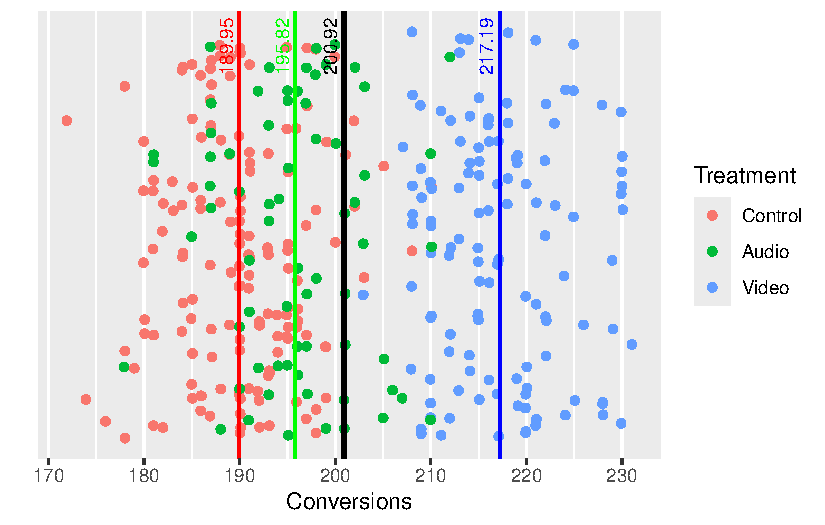
\includegraphics[keepaspectratio]{Anova_files/figure-pdf/fig-treatmentmeans-1.pdf}}

}

\caption{\label{fig-treatmentmeans}Treatment Means and Grand Means with
Data Distribution}

\end{figure}%

\textbf{Can we scientifically determine whether these observed
differences are statistically significant?}

\section{Why Not Use Pairwise A/B
Tests?}\label{why-not-use-pairwise-ab-tests}

A tempting idea in this setting is to run multiple pairwise \textbf{A/B
Tests} to compare each design against the \emph{Control}:

\begin{itemize}
\item
  \textbf{Audio} vs.~\textbf{Control}
\item
  \textbf{Video} vs.~\textbf{Control}
\end{itemize}

While intuitive, this approach introduces big statistical concern:
increased risk of false positives (\emph{Type I Error}). That is, by
running multiple comparisons independently, we raise the chance of
incorrectly concluding that a difference exists when it does not.

Even if each individual test maintains a 5\% error rate
(\(\alpha = 0.05\)), the combined probability of making at least one
false discovery across two tests rises to:

\[1−(1−0.05)^2=0.0975\approx 10
\%\]

With more variations, the problem compounds quickly. For example, if we
had four treatments in addition to the \emph{Control}, the chance of a
false positive somewhere among those comparisons would rise to nearly
20\%:

\[1−(1−0.05)^2=0.1855\approx 20 \%\]

Clearly, this inflation of error makes multiple pairwise\\
\emph{A/B Tests} \textbf{statistically unreliable}.

\textbf{A Better Alternative:\\
Testing all treatments at once} instead of running several separate
tests. This is where \emph{Analysis of Variance} or short \emph{ANOVA}
comes in:

\begin{itemize}
\item
  \emph{ANOVA} allows to test one or more groups of variables
  simultaneously
\item
  \emph{ANOVA} avoids the pitfalls of multiple testing
\end{itemize}

However, if the ANOVA result is significant, we know only that at least
one, but not which one(s) of the variables are significant. Afterward,
more testing is needed to find out which variable is significant.

\section{Regression and ANOVA}\label{regression-and-anova}

One way to approach \emph{ANOVA} is through regression analysis. The
idea is simple: if any of the treatment types (\emph{Audio} or
\emph{Video}) has an impact on conversions, then including these
variables in a regression model should improve its explanatory power.

This is exactly what we explore below. We fit a linear model with
\textbf{Treatment} as a categorical predictor of \textbf{Conversions}:

\[Conv_i=\beta_1 Audio_i+\beta_2 Video_i+ \beta_0\] Here, \(Audio_i\)
and \(Video_i\) are dummy variables for group membership. The
\textbf{Control group} is omitted and serves as the \textbf{reference
category}.

The code below runs the analysis in \emph{R}, stores the model in the
object \texttt{ModelLM}, and displays the summary output in
Table~\ref{tbl-LM} with \texttt{summary()}.

\begin{Shaded}
\begin{Highlighting}[]
\NormalTok{ModelLM }\OtherTok{=} \FunctionTok{lm}\NormalTok{(Conversions }\SpecialCharTok{\textasciitilde{}}\NormalTok{ Treatment, }\AttributeTok{data =}\NormalTok{ DataWeb)}

\FunctionTok{summary}\NormalTok{(ModelLM) }\SpecialCharTok{|\textgreater{}} 
\NormalTok{broom}\SpecialCharTok{::}\FunctionTok{tidy}\NormalTok{() }\SpecialCharTok{|\textgreater{}} 
\FunctionTok{kable}\NormalTok{(}\AttributeTok{caption=}\StringTok{"Output from the Linear Regression"}\NormalTok{) }\SpecialCharTok{|\textgreater{}} 
\FunctionTok{kable\_styling}\NormalTok{(}\AttributeTok{full\_width =} \ConstantTok{FALSE}\NormalTok{, }\AttributeTok{position =} \StringTok{"center"}\NormalTok{)}\SpecialCharTok{\%\textgreater{}\%}
\FunctionTok{scroll\_box}\NormalTok{(}\AttributeTok{width =} \StringTok{"600px"}\NormalTok{)}
\end{Highlighting}
\end{Shaded}

\begin{longtable}[t]{lrrrr}

\caption{\label{tbl-LM}Output from the Linear Regression}

\tabularnewline

\\
\toprule
term & estimate & std.error & statistic & p.value\\
\midrule
(Intercept) & 189.953642 & 0.5404799 & 351.453643 & 0\\
TreatmentAudio & 5.869887 & 0.9699452 & 6.051772 & 0\\
TreatmentVideo & 27.233349 & 0.8066819 & 33.759714 & 0\\
\bottomrule

\end{longtable}

At first glance, the \emph{t-values} for the treatment coefficients may
suggest statistical significance. However, due to the \textbf{multiple
testing problem}, we cannot rely on these individual \emph{t-tests} for
a \emph{multi-variable} comparison. Doing so would increase the risk of
an inflated \emph{Type I error} --- falsely concluding that a difference
exists when it does not.

\subsection{From Regression to ANOVA}\label{from-regression-to-anova}

So, if multiple \emph{t-test} are not an option:

\textbf{What can we do instead?}

Rather than testing each treatment effect separately, we assess their
combined influence on the model. In other words:

\textbf{Does adding the Treatment variables simultaneously improve the
model vs.~no treatment effect at all?}

This is precisely what \emph{ANOVA} measures in the context of
regression --- it compares the \textbf{explained variance of the full
model (with Treatment)} to a \textbf{restricted model (intercept-only in
our case)} using an \textbf{F-test.}

The \textbf{restricted model} model can be written like this:

\[
Conv_i=\beta_0 \qquad \mbox{ with: } \quad\beta_0=\frac{\sum_{i=1}^N Conv_i}{N}
\]

In other words, the \emph{restricted model} predicts every observation
using only the \textbf{Grand Mean} (mean of all \(Conversions\)).

To quantify the improvement of the \emph{Full} model over the
\emph{Restricted} model based on the Total Sum of Squared Errors
(\(SSE\)), we calculate the \emph{F-value} as follows:

\begin{equation}\phantomsection\label{eq-FValueOrg}{
F = \left(\frac{SSE_{restr}-SSE_{full}}{df_{restr}-df_{full}} \right ) \div
     \left(\frac{SSE_{full}}{df_{full}} \right )
}\end{equation} \[
\Longleftrightarrow\] \begin{equation}\phantomsection\label{eq-FValue}{
 F = \overbrace{\frac{SSE_{restr}-SSE_{full}}{SSE_{full}}}^{
\begin{array}{c}\text{Proportional Improvement}\\
                \text{(restr. to full model)}
\end{array}} \cdot
   \overbrace{\frac{df_{full}}{df_{restr}-df_{full}}}^{C_{onst}}
}\end{equation}

Source: \url{https://online.stat.psu.edu/stat501/lesson/6/6.2}

\textbf{The larger the \(F-\)value, the more improves the full model
over the restricted model --- the more important are the treatments
(\emph{Audio},\emph{Video}) for conversions.}

\subsection{Break Down the F-Value
Formula}\label{break-down-the-f-value-formula}

\textbf{The Right Multiplier (is constant):}

\begin{quote}
The second term in the formula --- the right-hand multiplier --- is
constant once the experimental design is fixed. It depends only on the
degrees of freedom of the models:

\begin{itemize}
\tightlist
\item
  \textbf{Number of observations:} \(N = 342\)\\
\item
  \textbf{Degrees of freedom for the restricted model (intercept
  only):}\\
  \(df_{\text{restr}} = 342 - 1 = 341\)\\
\item
  \textbf{Degrees of freedom for the full model (intercept + 2
  treatments):}\\
  \(df_{\text{full}} = 342 - 3 = 339\)
\end{itemize}

\textbf{We can calculate \(C^{\text{onst}}\) as follows:}

\[
C^{\text{onst}} = \frac{df_{\text{full}}}{df_{\text{restr}} - df_{\text{full}}}
= \frac{342 - 3}{(342 - 1) - (342 - 3)} 
= \frac{339}{2}
\]
\end{quote}

\textbf{The Left Multiplier: Model Improvement}

\begin{quote}
The left term in the formula captures how much better the full model is
in reducing the squared error:

\begin{equation}\phantomsection\label{eq-ProportionOfImprovement}{
\frac{SSE_{restr}-SSE_{full}}{SSE_{full}}
}\end{equation}
\end{quote}

\textbf{With the right multiplier of the F-value equation being
constant, it is only the left multiplier that determines if F is large
or not.}

\[
 F = \overbrace{\frac{SSE_{restr}-SSE_{full}}{SSE_{full}}}^{
\begin{array}{c}\text{Proportional Improvement}\\
                \text{(restr. to full model)}
\end{array}} \cdot
   \overbrace{\frac{df_{full}}{df_{restr}-df_{full}}}^{C_{onst}}
\]

\subsection{Calculating the SSEs in R}\label{calculating-the-sses-in-r}

To compute the \(SSE\) values for both models and derive the
F-statistic, we use the \texttt{anova()} function for a linear model:

\begin{Shaded}
\begin{Highlighting}[]
\NormalTok{ModelAnova}\OtherTok{=}\FunctionTok{anova}\NormalTok{(ModelLM)}
\end{Highlighting}
\end{Shaded}

The code below outputs the related \emph{ANOVA} table and adds a row for
the \emph{restricted model} (Intercept).

\begin{Shaded}
\begin{Highlighting}[]
\NormalTok{ModelAnovaRestr}\OtherTok{=}\FunctionTok{anova}\NormalTok{(}\FunctionTok{lm}\NormalTok{(Conversions}\SpecialCharTok{\textasciitilde{}}\DecValTok{1}\NormalTok{, }\AttributeTok{data=}\NormalTok{DataWeb))}

\NormalTok{FancyOutput}\OtherTok{=}\FunctionTok{rbind}\NormalTok{(broom}\SpecialCharTok{::}\FunctionTok{tidy}\NormalTok{(ModelAnovaRestr), }
\NormalTok{                  broom}\SpecialCharTok{::}\FunctionTok{tidy}\NormalTok{(ModelAnova)) }\SpecialCharTok{|\textgreater{}} 
                  \FunctionTok{select}\NormalTok{(}\SpecialCharTok{{-}}\NormalTok{p.value)}
\NormalTok{FancyOutput[}\DecValTok{1}\NormalTok{,}\DecValTok{1}\NormalTok{]}\OtherTok{=}\StringTok{"Intercept (ModelRestr)"}
\NormalTok{FancyOutput[}\DecValTok{3}\NormalTok{,}\DecValTok{1}\NormalTok{]}\OtherTok{=}\StringTok{"Residuals (ModelFull)"}
\FunctionTok{colnames}\NormalTok{(FancyOutput)}\OtherTok{=}\FunctionTok{c}\NormalTok{(}\StringTok{"Term"}\NormalTok{,}\StringTok{"df"}\NormalTok{, }\StringTok{"SSE"}\NormalTok{,}\StringTok{"MeanSq"}\NormalTok{,}\StringTok{"F{-}Value"}\NormalTok{)}
\FunctionTok{kbl}\NormalTok{(FancyOutput, }\AttributeTok{caption =} \StringTok{"Ammended anova() Output"}\NormalTok{) }\SpecialCharTok{|\textgreater{}} 
   \FunctionTok{kable\_styling}\NormalTok{(}\AttributeTok{full\_width =} \ConstantTok{FALSE}\NormalTok{, }\AttributeTok{position =} \StringTok{"center"}\NormalTok{)}\SpecialCharTok{\%\textgreater{}\%}    \FunctionTok{scroll\_box}\NormalTok{(}\AttributeTok{width =} \StringTok{"600px"}\NormalTok{)                 }
\end{Highlighting}
\end{Shaded}

\begin{table}

\caption{\label{tbl-ANOVA}}

\centering{

\centering
\caption{Ammended anova() Output}
\centering
\begin{tabular}[t]{l|r|r|r|r}
\hline
Term & df & SSE & MeanSq & F-Value\\
\hline
Intercept (ModelRestr) & 341 & 67426.54 & 197.7318 & NA\\
\hline
Treatment & 2 & 52473.28 & 26236.6419 & 594.8016\\
\hline
Residuals (ModelFull) & 339 & 14953.26 & 44.1099 & NA\\
\hline
\end{tabular}

}

\end{table}%

In the ANOVA output generated by \texttt{anova(ModelLM)}, the
\textbf{F-value} is already reported. However, we will recalculate it
below to illustrate the procedure \emph{under the hood} of the
\texttt{anova()} function.

\begin{center}\rule{0.5\linewidth}{0.5pt}\end{center}

\textbf{Step 1:}\\
The \textbf{Sum of Squared Errors} for the \textbf{restricted model},
which includes only the intercept (i.e., the grand mean of conversions),
is found in the \textbf{first row} of the ANOVA Table~\ref{tbl-ANOVA} ,
under the \(SSE\) column \((SSE_{\text{restr}} = 67,\!426)\).

\textbf{Step 2:}\\
The \textbf{Sum of Squared Errors} for the \textbf{full model}, which
includes the predictors \emph{Audio} and \emph{Video}, is listed in the
\textbf{Residuals} row (third row) of Table~\ref{tbl-ANOVA}
(\(SSE_{\text{full}} = 14,\!953\)).

\begin{quote}
🔍 \textbf{Note:} The first row of the Table~\ref{tbl-ANOVA} (labeled
\emph{Intercept}) is included primarily for convenience and
interpretability. However, all values required to compute the
F-statistic using Equation~\ref{eq-FValue} can be derived entirely from
the \textbf{second and third rows} which is the output produced by
\texttt{anova()}.

Specifically:

\begin{itemize}
\tightlist
\item
  \(SSE_{restr}-SE_{full}=67,\!426-14,\!953=52,\!473.28\) and
\item
  \(df_{restr}-df_{full}= 341-339=2\)
\end{itemize}

are both reported in row 2 of Table~\ref{tbl-ANOVA}.
\end{quote}

\textbf{Step 3:}\\
We now plug the values from Step 1 and Step 2 together with the related
degrees of freedom into the F-statistic formula from
Equation~\ref{eq-FValue}:

\[
F =
\underbrace{\frac{SSE_{\text{restr}} - SSE_{\text{full}}}{SSE_{\text{full}}}}_{
\begin{array}{c}
\text{Proportional Improvement} \\
\text{(restr. to full model)}
\end{array}
}
\cdot
\underbrace{\frac{df_{\text{full}}}{df_{\text{restr}} - df_{\text{full}}}}_{\text{Constant}}
\]

Plugging in the values we get:

\[
F =
\underbrace{\frac{67,\!426 - 14,\!953}{14,\!953}}_{
\approx 3.51
}
\cdot
\underbrace{\frac{339}{341-339}}_{= 169.5}
= 3.51 \cdot 169.5
\approx \boxed{594.80}
\]

The sum of squared errors (\(SSE\)) in the restricted model is
approximately \textbf{3.5 times larger} than in the full model. Thus
reflecting a big improvement through incorporating the treatment effects
(\emph{Audio} and \emph{Video}).

Multiplying this improvement factor by the constant \((169.5)\) yields
the \textbf{F-value of 594.8}, as reported in the ANOVA output. This
same value also appears in the \texttt{summary()} output for the linear
regression model, confirming consistency across both methods of
evaluation.

\section{F-value: When is Large Large Enough for Significance (needs
editing work by
CL!)}\label{f-value-when-is-large-large-enough-for-significance-needs-editing-work-by-cl}

In the previous section we derived an F-value of \(F=594.8\) and an
F-value of that the \textbf{sum of squared errors} in the restricted
model was approximately \textbf{3.5 times larger} than in the model that
included the treatment groups: \emph{Audio}, \emph{Video}, and
(implicitly) \emph{Control}.

This suggests that the chance of all three group means being equal ---
and thus, their inclusion in the \emph{full model} having no impact ---
is \textbf{extremely small}.

Still, in order to make a \textbf{scientific claim}, we need to test
this assumption formally by stating and rejecting an (admittedly
ridiculous) null hypothesis:

\[
\begin{align}
& \text{Hypothesis 0:}\\
\\
&Mean(Conv_{Control})=Mean(Conv_{Audio})=Mean(Conv_{Video})
\end{align}
\] If \textbf{Hypothesis 0} were true, then including the treatment
variables in the model would \textbf{not} reduce the error. The full
model would perform just as poorly as the restricted one --- meaning the
F-statistic should be around \textbf{1}. Thus, we can simplify our
\textbf{Hypothesis 0} to:

\[
\begin{align}
&\text{Hypothesis 0:}\\
\\
&F=1
\end{align}
\]

\begin{quote}
🤓 \textbf{Only for the curious reader:} You might wonder --- should the
F-value be 0 under \emph{Hypothesis 0}? After all, if there is no
improvement, the numerator of the F-value (i.e.,
\(SSE_{\text{restr}} - SSE_{\text{full}}\)) in Equation~\ref{eq-FValue}
would be zero.

That intuition is partly correct: if \emph{Hypothesis 0} is true, the
\textbf{expected value} of this difference is indeed zero: \[
E(SSE_{\text{restr}} - SSE_{\text{full}}) = 0
\]

However, the \textbf{variance} of
\((SSE_{\text{restr}} - SSE_{\text{full}})\) is \textbf{not zero},
because repeated sampling would yield slightly different SSEs for each
model. In fact, \(SSE_{\text{restr}} - SSE_{\text{full}}\) if
\emph{Hypothesis 0} is true:
\[Var(SSE_{restr}-SSE_{Full})=Var(SSE_{Full})\]

Since we find these two variances in the divident and divisor of
Equation~\ref{eq-FValueOrg}, \(F=1\) --- if the \emph{Hypothesis 0} is
true.
\end{quote}

Although we obtained an F-value of \(F = 594.8\), we cannot immediately
rule out the possibility that this result was due to \textbf{random
chance} --- that is, a fluke in our sample --- and that the true
\emph{F-value} might still be 1.

\textbf{However, we can assess how (un)likely it would be to obtain such
a high \emph{F-value} if \emph{Hypothesis 0} were true.}

To do this, we calculate a \textbf{p-value}, which represents the
probability of observing an \emph{F-value} as extreme as the one we
found --- \textbf{assuming Hypothesis 0 is true}.

To compute the \emph{p-value} from the \emph{F-distribution}, we need to
know the degrees of freedom for the two variances we compare according
to Equation~\ref{eq-FValue}. The first one is \(df_{restr}-df_{full}\)
(341-339=2) and the second one is \(df_{full}\) (339).

Since we trying to reject the hypothesis with a sample \emph{F-value}
that is far to the right of \(F=1\) we are performing a
\emph{right-tail} test. Below is the related code and the result:

\begin{Shaded}
\begin{Highlighting}[]
\NormalTok{PValue}\OtherTok{=}\FunctionTok{pf}\NormalTok{(}\FloatTok{594.8}\NormalTok{, }\AttributeTok{df1 =} \DecValTok{2}\NormalTok{, }\AttributeTok{df2 =} \DecValTok{339}\NormalTok{, }\AttributeTok{lower.tail =} \ConstantTok{FALSE}\NormalTok{)}
\end{Highlighting}
\end{Shaded}

\begin{Shaded}
\begin{Highlighting}[]
\FunctionTok{cat}\NormalTok{(}\StringTok{"The probability to get such an high F{-}Value, }\SpecialCharTok{\textbackslash{}n}\StringTok{if the Hyppothesis 0 were true,}
\StringTok{is (in scientific notation):}\SpecialCharTok{\textbackslash{}n}\StringTok{"}\NormalTok{, PValue)}
\end{Highlighting}
\end{Shaded}

\begin{verbatim}
The probability to get such an high F-Value, 
if the Hyppothesis 0 were true,
is (in scientific notation):
 1.352198e-111
\end{verbatim}

\begin{Shaded}
\begin{Highlighting}[]
\FunctionTok{cat}\NormalTok{(}\StringTok{"The probability to get such an high F{-}Value, }\SpecialCharTok{\textbackslash{}n}\StringTok{if the Hyppothesis 0 were true,}
\StringTok{is (written out):}\SpecialCharTok{\textbackslash{}n}\StringTok{"}\NormalTok{, }\FunctionTok{format}\NormalTok{(PValue, }\AttributeTok{scientific =} \ConstantTok{FALSE}\NormalTok{))}
\end{Highlighting}
\end{Shaded}

\begin{verbatim}
The probability to get such an high F-Value, 
if the Hyppothesis 0 were true,
is (written out):
 0.000000000000000000000000000000000000000000000000000000000000000000000000000000000000000000000000000000000000001352198
\end{verbatim}

With such a low probability for a \emph{Type-1} error we can safely
state:

\textbf{One of our treatments, did significantly influence the
conversions}

To identify which treatment \emph{Audio} or \emph{Video} (or possibly
both) influenced conversions, we need further testing, which exceeds the
scope of this article.

Happy analytics!




\end{document}
